%\todo[inline]{existing game research?? own section?}

\section{Games and the Virtual Reality}
\label{sec:gamesNvr}

To catch a brief insight into games that both support playing with or without HMD and to further introduce research aspects of the following section this paragraph is intended to list a few differences, similarities and uniqueness within games. An overview of these games can be found in \textbf{Table~\ref{tab:popularGames}}, where some properties of these games are listed. 

Starting with \textit{Minecraft}. an open world sandbox game where the player controls his playable character by navigating with the keyboard or game controller. The goal is to mine blocks of different material and craft them into objects which he will need to complete the game. As it is an open world game the player can move to different areas in order to gather some items needed. 

A disadvantage of this game is the locomotion method needed in order to move around the world. Since the game has not many stationary tasks and it depends on the ability of the user to move around it holds greater potential for the virtual reality sickness occurring when exposed to a virtual environment and has similar symptoms to motion sickness.

\begin{figure}
	\centering
	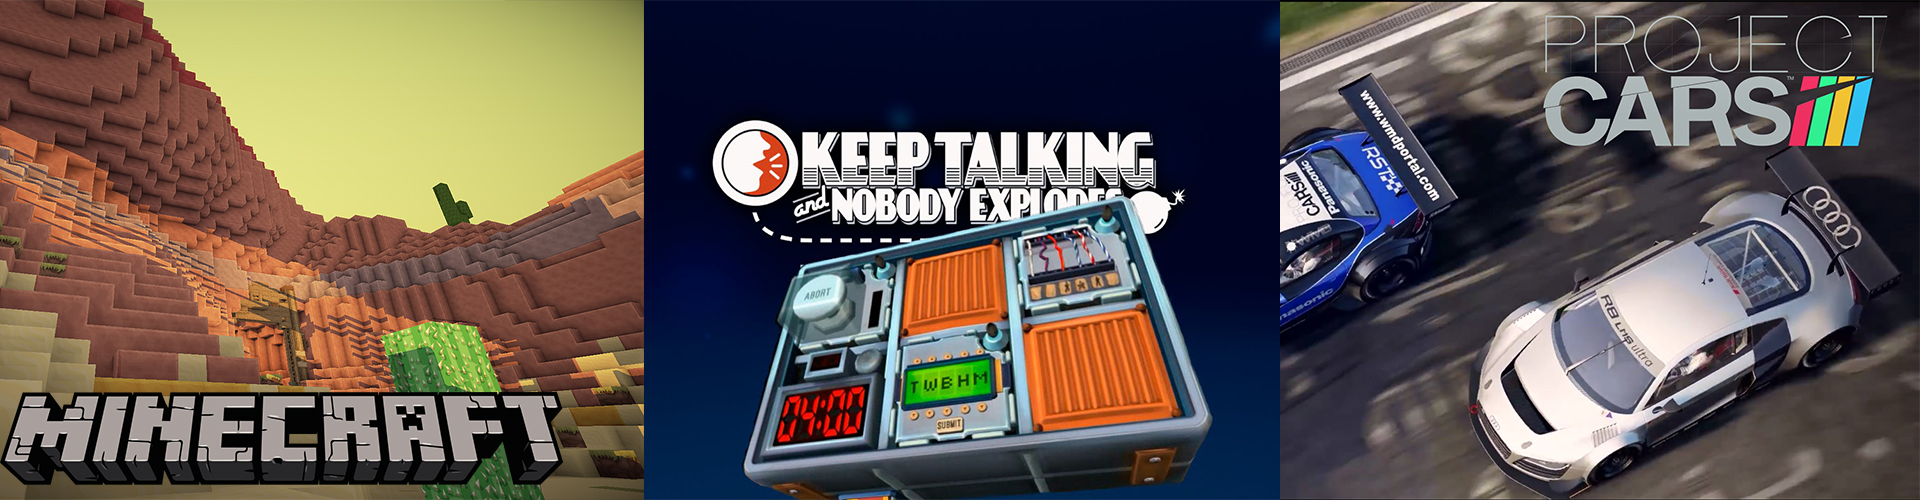
\includegraphics[width=0.99\columnwidth]{./figures/banner}
	\caption[banner]{The three presented games. FLTR Minecraft, Keep talking and nobody explodes and Project CARS. Each game offers native VR Support on multiple devices and has different interaction methods for locomotion.\footnotemark}~\label{fig:banner}
\end{figure}
\footnotetext{
	\textcopyright~Mohjang, Steel Crate Games, Slightly Mad Studios, [Online; accessed January 04., 2017],[Digitally edited] \url{https://pixabay.com/p-354458} \url{https://i.ytimg.com/vi/Apwa_ksMvM0/maxresdefault.jpg} \url{https://i.ytimg.com/vi/RggvBJ2ANWo/maxresdefault.jpg} \ccbyncsa
}

Another game is \textit{Keep Talking and Nobody Explodes} a puzzle game where one player has to describe and disarm a virtual explosive charge in a given time. His team members, who cannot see the bomb, have to explain what player one has to do in order to disarm the bomb and to save his and the team members lives. The game mechanics are different from those of Minecraft. The player wearing the HMD has a stationary task and just needs to interact with objects in his direct vicinity. 

Because of this only natural locomotion the peril of becoming sick is very weakly present.

Project CARS is a racing simulation for Microsoft Windows, PlayStation 4, and Xbox One. It offers standard racing simulation whilst also providing the kind of advanced features usually reserved for PC-only simulators.

The locomotion is solely a cockpit locomotion, meaning that the player is sitting in a virtual car and steering with different interfaces. Because of the visual stimuli of moving inside a car but because neither the vibration nor the acceleration is noticeable the user is weakly prone to becoming VR sick.

\begin{table}%[h]
	\caption{Popular games played in late 2016. The games offer a regular play mode, using the monitor, and a VR play mode with both the Oculus Rift and the HTC Vive}~\label{tab:popularGames}
	
	%{}\fontfamily{pcr}\selectfont
	\renewcommand{\arraystretch}{1.3}% for the vertical padding
	\begin{tabular*}{\columnwidth}{ p{33mm} l r l }
		Gametitle & Genre\footnotemark & \parbox[c][2.2em][t]{2cm}{\begin{flushright}$\dfrac{Players}{Month}$(\footnotemark)\end{flushright}} & LM\footnotemark \\
		\hline
		Minecraft & RPG & 990 K & ALM \\
		Keep Talking and \newline Nobody Explodes & Puzzle & 153.3 & NLM \\
		Project CARS & Racing & 1.01 K & CLM\\
	\end{tabular*}
	%}
	
\end{table}

\footnotetext[3]{RPG: Role-Playing Game}
\footnotetext[4]{\url{http://steamcharts.com}, accessed Jan. 3., 2017}
\footnotetext[5]{Types of Locomotion (LM): Natural Locomotion (NLM), Cockpit Locomotion (CLM), Artificial Locomotion (ALM) See also: Section\ref{sec:locomotion}:~Locomotion}
%\todo[inline]{Die footnotes werden nicht richtig nummeriert... von hand fixen bei submission!?}

\subsection{Popularity Of VR Games}
Since the beginning of virtual reality in the 20th century there has been a huge potential to include the user in a virtual environment. Some systems have been developed in the past century that simplify some processes of work for different disciplines. 

Games have just lately adopted the potential for this immerse form of gaming. VR offers new dimensions to include the player into a game world and to tell stunning stories.

Using a virtual environment to show worlds to players has the great advantage of giving them the feeling of being in the middle of the event, but the game has very limited possibilities to tell stories with much variety. Meaning that the game can not change perspectives as easy. While games that do not use VR can handle attention themselves by just moving the camera. These games can show views from other perspective without worrying about the user being confused too much. VR-Games need another way to handle interaction, i.e. the user has to hold some kind of controller interface to tell the system what he wants to do. Games outside of VR have similar interface problems but the process has been researched more than the interaction with VR-Games. Simultaneously VR games require a much more active way of interaction, because the user has to complete different tasks as he is playing the game. This can be a negative point for people who would just rather enjoy a game than have a minor workout while playing.
%			
%pro vr: immerse, active, intuitive, innovative.
%contra vr: active, expensive, hard(er) to develop games
%
%Why VR games are as popular as they are
%
%Why are VR games not as popular as regular games. Are the prices for the equipment too high or are the Games just not developed enough?
%
%\todo[inline]{JF: Auch oder vielleicht sogar mehr: Wieso nicht? Ist es nur dass die Technologie noch nicht verbreitet genug ist? Machen die Spiele was anders? Funktionieren traditionelle Spiele nicht einfach so in VR? etc.}

\subsection{Motivation In Games}

\begin{figure}
	\centering
	
\includegraphics[width=0.9\columnwidth]{./figures/placeholder}
	\caption[blabla]{Lorem Ipsum dolor sit amet bla bla bla, foo , bar bla blubb fooooooo bla bla bla bla bla bla bla}~\label{fig:foobar3}
\end{figure}


What Motivation can VR offer that other Games cannot offer. What motivation can normal games offer, that vr-games cannot offer.

motivation of players: (talk)\footnote{"Gamer Motivation Profile Findings - \#GamesUR US Conference 2016" Quantic Foundry Website, March, 25., 2015, accessed November 05., 2016, \url{http://quanticfoundry.com/2016/04/07/gdc-talk/}}
\begin{itemize}
	\item action - people who like the thrill and the challenge
	\item social - people who like to be together with others, socialize and help others
	\item mastery - -making complex decisions
	\item achievement - those who want to achieve something and show others that they are good, or those who want to compare to others
	\item immersion - those who want to (temporarily) escape the 'real' world and who want to feel immersed into a game
	\item creativity - those who want to be creative, build something .. making the game your own in any way. 
	\item \textbf{age} - differences between the young generation and the old one (older people mostly have another point of view on things and have other motivation) But also the younger generation, grown up with video games will have a different motivation than the 'older' generation today. (because of the constant companionship of games)
\end{itemize}

3 clusters 

action-social

mastery-achievement

immersion-creativity

\subsection{Input Techniques}
Nicht so spezifisch darauf eingehen, welche eingabemethoden existieren, sondern viel mehr auf Sec 12 Further research trends!

Vielleicht kann diese Section sogar in eine 14 zurück verlagert werden, da nicht wirklich notwendig eigenes Kapitel zu erstellen 
Oculus Rift

HTC Vive

Samsung Gear

playstation vr

\textcolor{red}{google: best VR games 2016: titles you cant miss for ... -> compare Oculus to PS, Oculus to Vive etc. -> \url{http://www.wareable.com/gaming/top-vr-games-for-oculus-rift-project-morpheus-gear-vr-and-project-cardboard}}

\url{http://newatlas.com/best-vr-headsets-comparison-2016/45984/}

Dancing in front of a camera. XBox camera stuff

what research has been done. how can input be changes. what adjustments are possible. what adjustments are necessary. How can a user be teached what to do if some things happen. what generic input of interaction methods can be defined beween systems.

what other channel of interaction can be used (sound, video)
